
\documentclass[11pt,a4paper]{report}
\usepackage[a4paper,margin=0.82in,headheight=15pt]{geometry}
\usepackage[T1]{fontenc}
\usepackage{lmodern}
\usepackage{microtype}
\usepackage{graphicx}
\usepackage{tikz}
\usetikzlibrary{arrows.meta,positioning,shapes.geometric,shapes.misc,fit,calc,backgrounds}
\usepackage{float}
\usepackage{array}
\usepackage{booktabs}
\usepackage{longtable}
\usepackage{tabularx}
\usepackage{amsmath}
\usepackage{enumitem}
\usepackage{fancyhdr}
\usepackage[hidelinks]{hyperref}
\usepackage{xcolor}
\usepackage{caption}
\usepackage{titlesec}
\setlength{\parskip}{4pt}
\setlength{\parindent}{0pt}
\renewcommand{\arraystretch}{1.18}
\setlist[itemize]{leftmargin=1.5em,itemsep=2pt,topsep=3pt}
\setlist[enumerate]{leftmargin=1.7em,itemsep=3pt,topsep=3pt}
\pagestyle{fancy}
\fancyhf{}
\fancyhead[L]{UCS503 -- Software Engineering}
\fancyhead[R]{SmartCross -- EST Evaluation}
\fancyfoot[C]{\thepage}
\hypersetup{pdftitle={SmartCross -- End-Semester Evaluation},pdfauthor={Moksh, Sandeep Yadav, Gagandeep Singh}}
\definecolor{scblue}{RGB}{25,74,120}
\definecolor{scgray}{RGB}{242,245,248}
\definecolor{scgreen}{RGB}{225,242,231}
\definecolor{scorange}{RGB}{255,239,218}
\tikzset{
  nodebox/.style={draw=black!70,rounded corners=3pt,fill=scgray,align=center,
    minimum height=0.78cm,minimum width=2.35cm,text width=2.5cm,font=\small,inner sep=5pt},
  smallbox/.style={draw=black!70,rounded corners=3pt,fill=white,align=center,
    minimum height=0.62cm,minimum width=1.8cm,text width=2.0cm,font=\scriptsize,inner sep=4pt},
  actorbox/.style={draw=black!70,rounded corners=2pt,fill=white,align=center,
    minimum height=0.65cm,minimum width=1.6cm,text width=1.7cm,font=\small,inner sep=4pt},
  decision/.style={diamond,draw=black!70,fill=scorange,align=center,aspect=2,
    inner sep=2pt,font=\scriptsize,text width=1.7cm},
  dbbox/.style={cylinder,shape border rotate=90,draw=black!70,fill=scgreen,
    aspect=0.25,minimum height=1.0cm,minimum width=2.0cm,align=center,font=\small},
  usecase/.style={ellipse,draw=black!70,fill=white,align=center,
    minimum width=2.5cm,minimum height=0.72cm,text width=2.6cm,font=\scriptsize,inner sep=3pt},
  arr/.style={-{Latex[length=2.2mm]},thick},
  darr/.style={-{Latex[length=2.2mm]},thick,dashed},
  labeltxt/.style={font=\scriptsize,fill=white,inner sep=1pt}
}
\newcommand{\project}{\textbf{SmartCross}}
\newcommand{\statusnote}{\textit{All crossing states in this project are software predictions; the system is not connected to physical gate-position sensors.}}
\begin{document}

% TITLE PAGE
\begin{titlepage}
\centering
\vspace*{1.0cm}
{\Large\bfseries UCS503 -- SOFTWARE ENGINEERING\par}
\vspace{1.5cm}
{\Huge\bfseries SmartCross\par}
\vspace{0.35cm}
{\Large Real-Time Railway Crossing Monitoring and Prediction System\par}
\vspace{1.4cm}
{\large\bfseries End-Semester Evaluation Report\par}
\vspace{1.2cm}
{\large
\texttt{1024030925} Moksh\\[5pt]
\texttt{1024030312} Sandeep Yadav\\[5pt]
\texttt{1024030314} Gagandeep Singh\par}
\vspace{0.9cm}
{\large Group: 2C23 \quad BE Third Year\par}
\vspace{1.0cm}
{\large\bfseries Faculty Advisor\par}
{\large Dr. Jhonsy Bansal\par}
\vfill
{\large Computer Science and Engineering Department\par}
{\large Thapar Institute of Engineering and Technology, Patiala\par}
{\large November 2026\par}
\end{titlepage}

\pagenumbering{roman}
\tableofcontents
\listoffigures
\listoftables
\clearpage
\pagenumbering{arabic}

% CHAPTER 1
\chapter{Introduction}
\section{Background and Context}
Railway level crossings are shared points between road traffic and railway traffic. Road users approaching a crossing may not know whether a train is approaching, how soon it may reach the crossing, or how long the crossing may remain unavailable. Conventional train-tracking information is useful, but a train's location alone does not directly communicate the expected effect on a particular road crossing.

\project{} is a railway-crossing monitoring and prediction web application developed for the Patiala--Dhablan railway corridor in Punjab. It combines train timetable information, live train observations from the RailRadar service, railway-track geometry, prediction logic and a real-time web interface. The application converts train movement into crossing-specific estimates and displays an understandable predicted state to road users.

The current project focuses on four crossings: Phatak 19 (Station Approach), Phatak 20 (Sirhind Road), Phatak 23 (Model Town Extension) and Phatak 24 (Dhablan Approach). The software models their order and distance along the railway corridor rather than treating them as unrelated map points.

\section{Problem Statement}
A road user needs information about the crossing that they are approaching, not only the general location of a train. A useful system must therefore:
\begin{itemize}
  \item identify trains scheduled to pass through the monitored corridor;
  \item obtain live observations at an appropriate time while respecting API limits;
  \item estimate the train's position and arrival time at each relevant crossing;
  \item combine predictions from multiple trains without incorrectly showing a crossing as available;
  \item communicate changes to connected users quickly; and
  \item indicate uncertainty when live position data is stale or unavailable.
\end{itemize}

The project addresses these requirements through a backend prediction engine and a React-based monitoring interface. It is an advisory information system and does not control railway signalling or physical barriers.

\section{Project Objectives}
\begin{enumerate}
  \item Develop a web application for monitoring four railway crossings on the Patiala--Dhablan corridor.
  \item Integrate RailRadar train information and timetable data.
  \item Convert route-relative train position into along-track distance (chainage) for crossing-level ETA calculation.
  \item Use multiple prediction sources when fresh live position data is unavailable.
  \item Determine crossing states by aggregating the effects of all relevant trains.
  \item Deliver updated snapshots, status transitions and alerts through REST APIs and Socket.IO.
  \item Provide a simulation mode for controlled testing of train movement and exceptional scenarios.
  \item Store train, crossing, prediction, alert, event and evaluation information in MongoDB.
\end{enumerate}

\section{Scope and Limitations}
The implemented scope is limited to the configured Patiala--Dhablan corridor and the monitored train list maintained in system settings. Only monitored passenger trains with usable timetable or live data are covered. Unscheduled trains and freight trains are not predicted by the current implementation.

\statusnote{} The application predicts a crossing condition from train data and configurable thresholds. It does not measure the actual barrier position, issue railway operating commands, or guarantee that a road crossing is physically safe to enter. Estimated closure and reopening times may differ from actual railway operations.

% CHAPTER 2
\chapter{System Overview and Requirements}
\section{System Overview}
The application follows a modular client--server architecture. The React frontend requests an initial state through REST endpoints and receives subsequent updates through Socket.IO. The Node.js/Express backend coordinates the scheduler, RailRadar client, data normalizer, position resolver, corridor prediction engine, state machine, alert service and persistence layer. MongoDB stores reference data and operational records.

Two operating modes are supported:
\begin{itemize}
  \item \textbf{LIVE mode:} timetable scheduling controls when a monitored train is tracked and when RailRadar live polling is eligible.
  \item \textbf{SIMULATION mode:} simulated train movement is passed through the same normalisation, position resolution, prediction and state-transition pipeline. Simulated records are labelled separately.
\end{itemize}

\section{Functional Requirements}
\begin{longtable}{p{1.5cm}p{12.0cm}}
\toprule
\textbf{ID} & \textbf{Requirement}\\
\midrule
FR-01 & The system shall maintain the configured list of monitored trains and their corridor timetable information.\\
FR-02 & The scheduler shall begin live polling within the configured pre-entry window and stop after the configured post-clear window or when the train has left the corridor.\\
FR-03 & The system shall validate and normalize external train responses before using them.\\
FR-04 & The system shall resolve train position to a chainage value along the railway track.\\
FR-05 & The system shall calculate an ETA and closure/reopening estimates for each relevant crossing.\\
FR-06 & The system shall use a fallback prediction source when fresh live position is unavailable.\\
FR-07 & The system shall aggregate multiple train predictions into one predicted state per crossing.\\
FR-08 & The system shall suppress unstable state downgrades using confirmation timing (hysteresis).\\
FR-09 & The system shall expose crossing, train, prediction, alert and analytics information through REST endpoints.\\
FR-10 & The system shall broadcast snapshots, state transitions and alerts through Socket.IO.\\
FR-11 & The system shall support administrator authentication for protected settings and simulation controls.\\
FR-12 & The system shall support multi-train simulation scenarios and clearly distinguish simulated data from live data.\\
FR-13 & The system shall persist relevant operational information in MongoDB.\\
FR-14 & The system shall expose analytics for train frequency, speed, waiting estimates, prediction evaluation and API usage.\\
\bottomrule
\end{longtable}

\section{Non-Functional Requirements}
\begin{itemize}
  \item \textbf{Reliability:} malformed, missing, stale or unavailable train data must not be treated as a fresh measured position.
  \item \textbf{Performance:} the backend should calculate and publish updates promptly while limiting duplicate external requests.
  \item \textbf{Scalability:} corridor definitions and train mappings should be data-driven so that additional crossings can be configured.
  \item \textbf{Usability:} crossing state, ETA, prediction source and confidence should be understandable in the interface.
  \item \textbf{Security:} administrative routes require authentication; input validation, rate limiting and environment-based secrets are used.
  \item \textbf{Maintainability:} services are separated by responsibility and automated tests cover key prediction and integration behaviour.
\end{itemize}

\section{Users and Roles}
\begin{itemize}
  \item \textbf{Road user / viewer:} views the dashboard, map, crossing details, trains, alerts and analytics exposed by the application.
  \item \textbf{Administrator:} authenticates to manage monitored trains and thresholds, inspect operational metrics, switch modes and control simulations.
  \item \textbf{External data provider:} RailRadar supplies train timetable and live-status responses; it is an external dependency, not a SmartCross user.
\end{itemize}

% CHAPTER 3
\chapter{System Architecture and Design}
\section{High-Level System Architecture}
Figure~\ref{fig:architecture} represents the implemented architecture and the direction of the main data flows.

\begin{figure}[H]\centering
\resizebox{\textwidth}{!}{%
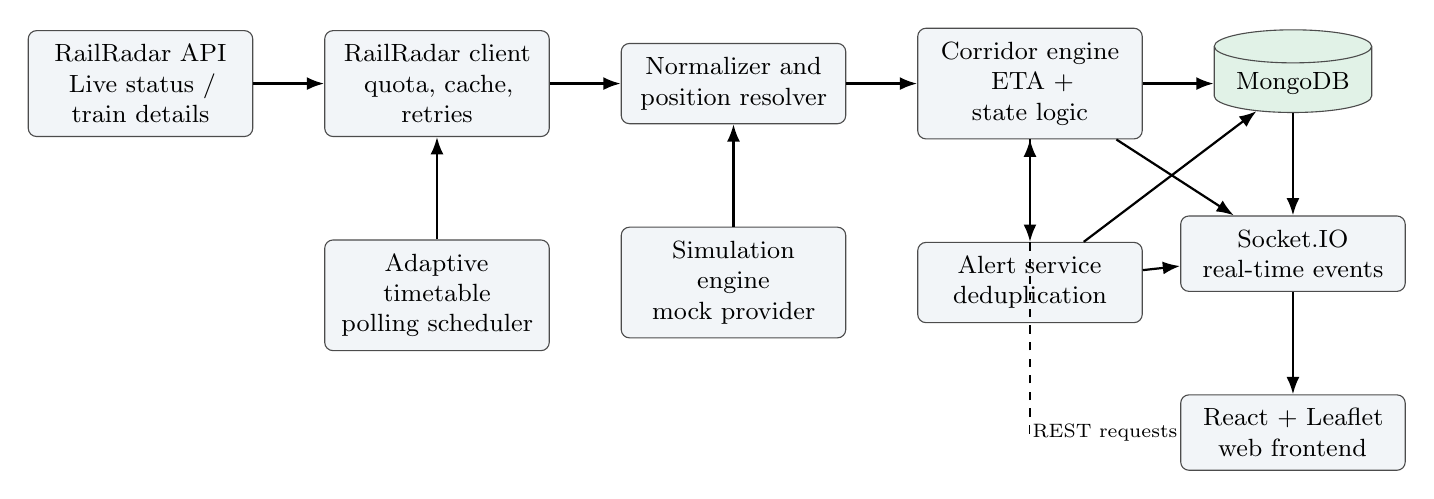
\begin{tikzpicture}[node distance=0.85cm and 0.9cm]
\node[nodebox] (rr) {RailRadar API\\Live status / train details};
\node[nodebox, right=of rr] (client) {RailRadar client\\quota, cache, retries};
\node[nodebox, right=of client] (norm) {Normalizer and\\position resolver};
\node[nodebox, right=of norm] (engine) {Corridor engine\\ETA + state logic};
\node[dbbox, right=of engine] (db) {MongoDB};
\node[nodebox, below=1.3cm of client] (sched) {Adaptive timetable\\polling scheduler};
\node[nodebox, below=1.3cm of norm] (sim) {Simulation engine\\mock provider};
\node[nodebox, below=1.3cm of engine] (alert) {Alert service\\deduplication};
\node[nodebox, below=1.3cm of db] (ws) {Socket.IO\\real-time events};
\node[nodebox, below=1.3cm of ws] (fe) {React + Leaflet\\web frontend};
\draw[arr] (sched) -- (client);
\draw[arr] (rr) -- (client);
\draw[arr] (client) -- (norm);
\draw[arr] (sim) -- (norm);
\draw[arr] (norm) -- (engine);
\draw[arr] (engine) -- (db);
\draw[arr] (engine) -- (alert);
\draw[arr] (alert) -- (db);
\draw[arr] (engine) -- (ws);
\draw[arr] (alert) -- (ws);
\draw[arr] (db) -- (ws);
\draw[arr] (ws) -- (fe);
\draw[darr] (fe.west) -| node[labeltxt,pos=0.25]{REST requests} (engine.south);
\end{tikzpicture}}
\caption{High-level architecture of SmartCross}
\label{fig:architecture}
\end{figure}

\section{Technology Stack}
\begin{longtable}{p{3.0cm}p{10.5cm}}
\toprule
\textbf{Layer} & \textbf{Technology / Responsibility}\\
\midrule
Frontend & React 18, Vite, React Router, Tailwind CSS, Leaflet / React-Leaflet and Recharts.\\
Backend & Node.js and Express.js; controllers, routes, middleware and modular services.\\
Database & MongoDB through Mongoose models and indexes.\\
External train data & RailRadar API for live train status and train/timetable information.\\
Track geometry & OpenStreetMap-derived railway geometry and corridor chainage.\\
Real-time communication & Socket.IO for snapshots, crossing updates, train updates, alerts and system status.\\
Testing & Jest, Supertest and socket.io-client based backend tests.\\
Deployment support & Dockerfiles, Docker Compose, health checks and Nginx frontend configuration.\\
\bottomrule
\end{longtable}

\section{Corridor and Crossing Model}
The corridor is represented using chainage: distance measured along the railway track from Patiala station. The configured order is Patiala $\rightarrow$ Phatak 19 $\rightarrow$ Phatak 20 $\rightarrow$ Phatak 23 $\rightarrow$ Phatak 24 $\rightarrow$ Dhablan.

\begin{table}[H]\centering
\caption{Configured Patiala--Dhablan corridor reference points}
\label{tab:corridor}
\begin{tabularx}{\textwidth}{c X r r r}
\toprule
\textbf{Point} & \textbf{Name} & \textbf{Latitude} & \textbf{Longitude} & \textbf{Chainage (m)}\\
\midrule
19 & Station Approach & 30.339583 & 76.398417 & 427\\
20 & Sirhind Road & 30.339667 & 76.392583 & 1,001\\
23 & Model Town Extension & 30.340222 & 76.366583 & 3,508\\
24 & Dhablan Approach & 30.339972 & 76.356778 & 4,449\\
DBN & Dhablan station & 30.337749 & 76.278590 & 11,957\\
\bottomrule
\end{tabularx}
\end{table}

The two configured crossing groups are Group A (Phataks 19 and 20) and Group B (Phataks 23 and 24). The application computes each crossing's own predicted closure window. It does not assume that the barriers in a group close simultaneously.

\section{Component Design}
The backend is separated into the following major components:
\begin{itemize}
  \item \textbf{RailRadar service:} API client, live train service, timetable service, normalizer and mock provider.
  \item \textbf{Scheduler:} builds per-train polling plans from timetable entry and exit times, known delay and configured windows.
  \item \textbf{GIS service:} converts route position into corridor chainage and calculates along-track distances.
  \item \textbf{Prediction service:} calculates ETA, applies fallback sources, smooths estimates and evaluates historical observations.
  \item \textbf{Corridor engine:} evaluates all active trains against all relevant crossings.
  \item \textbf{Gate state machine:} aggregates train impacts, applies priority and hysteresis, and emits transitions.
  \item \textbf{Alert and WebSocket services:} persist and broadcast deduplicated alerts and real-time updates.
  \item \textbf{Frontend:} renders dashboards, maps, train/crossing detail, alerts, analytics, settings, admin and simulation pages.
\end{itemize}

\section{Data Flow Diagram}
\begin{figure}[H]\centering
\resizebox{0.95\textwidth}{!}{%
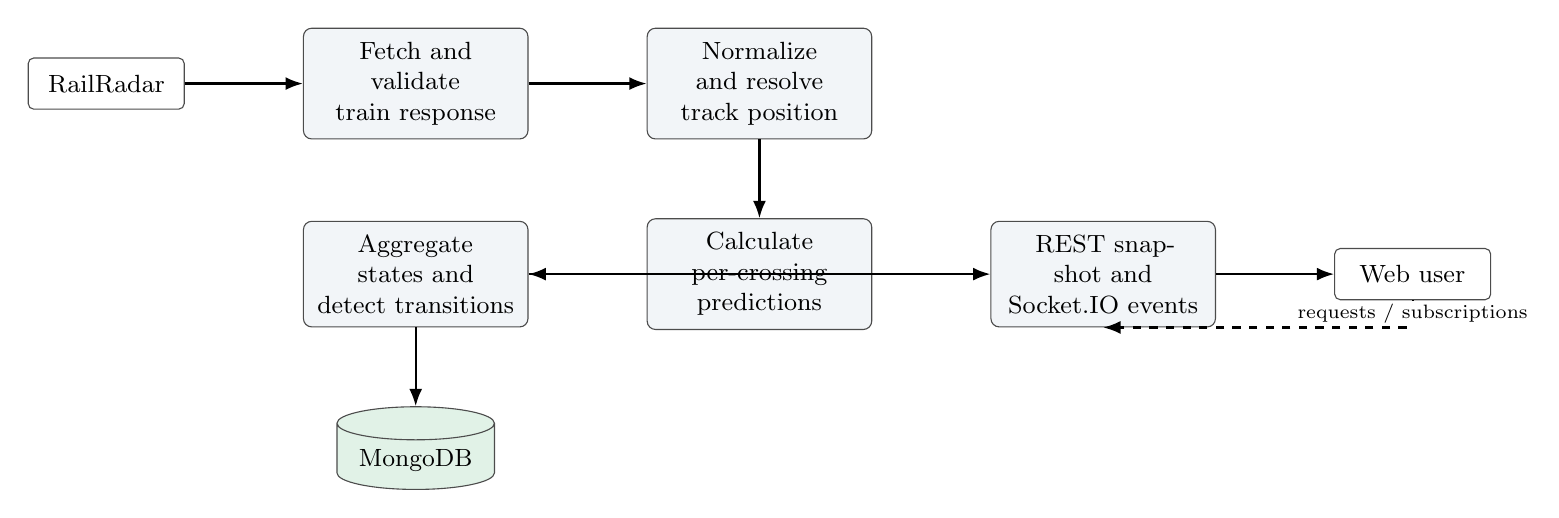
\begin{tikzpicture}[node distance=1.0cm and 1.5cm]
\node[actorbox] (provider) {RailRadar};
\node[nodebox, right=of provider] (p1) {Fetch and validate\\train response};
\node[nodebox, right=of p1] (p2) {Normalize and resolve\\track position};
\node[nodebox, below=of p2] (p3) {Calculate per-crossing\\predictions};
\node[nodebox, left=of p3] (p4) {Aggregate states and\\detect transitions};
\node[dbbox, below=of p4] (store) {MongoDB};
\node[nodebox, right=of p3] (p5) {REST snapshot and\\Socket.IO events};
\node[actorbox, right=of p5] (user) {Web user};
\draw[arr] (provider)--(p1);
\draw[arr] (p1)--(p2);
\draw[arr] (p2)--(p3);
\draw[arr] (p3)--(p4);
\draw[arr] (p4)--(store);
\draw[arr] (p4)--(p5);
\draw[arr] (p5)--(user);
\draw[darr] (user.south) |- node[labeltxt,pos=0.25]{requests / subscriptions} (p5.south);
\end{tikzpicture}}
\caption{SmartCross data processing flow}
\label{fig:dfd}
\end{figure}

\section{Sequence Diagram}
The sequence below shows a scheduled live polling cycle. In simulation mode, the simulation engine supplies mock RailRadar-format observations to the same normalizer and corridor engine.

\begin{figure}[H]\centering
\resizebox{\textwidth}{!}{%
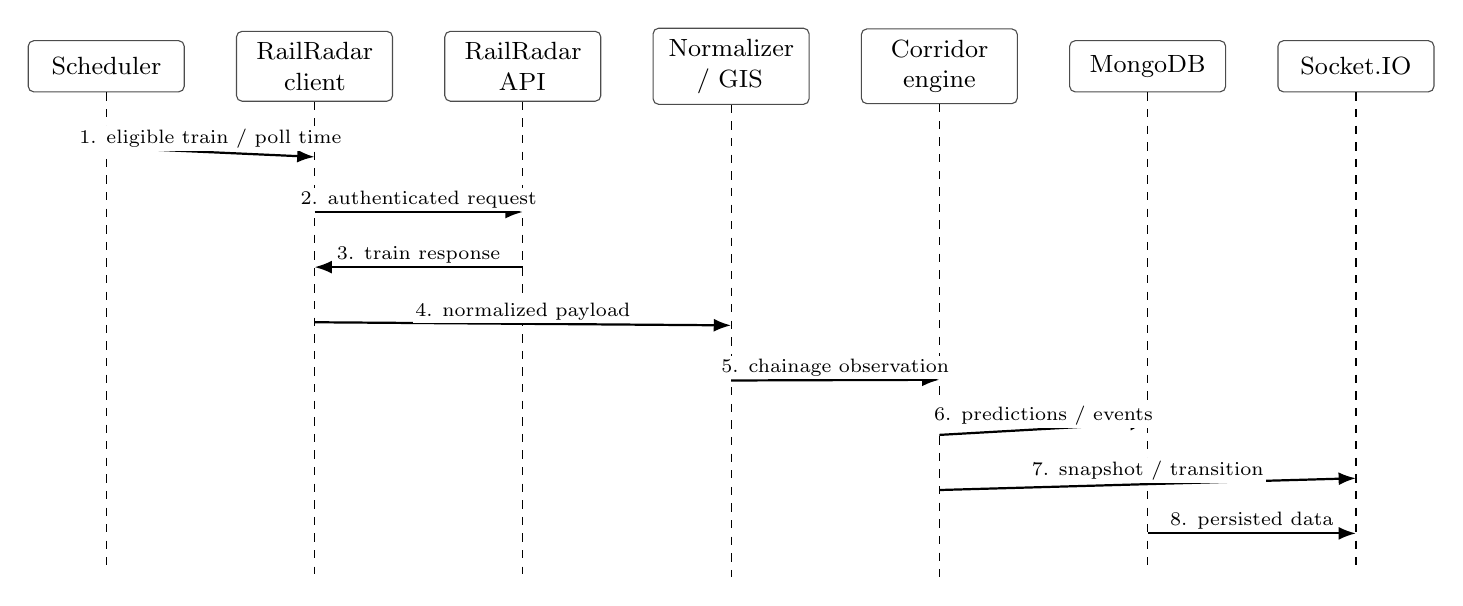
\begin{tikzpicture}[node distance=0.75cm and 0.65cm]
\node[actorbox] (sch) {Scheduler};
\node[actorbox, right=of sch] (api) {RailRadar client};
\node[actorbox, right=of api] (rr) {RailRadar API};
\node[actorbox, right=of rr] (res) {Normalizer / GIS};
\node[actorbox, right=of res] (eng) {Corridor engine};
\node[actorbox, right=of eng] (db) {MongoDB};
\node[actorbox, right=of db] (ws) {Socket.IO};
\foreach \n in {sch,api,rr,res,eng,db,ws}{
  \draw[dashed] (\n.south) -- ++(0,-6.0);
}
\draw[arr] ([yshift=-0.7cm]sch.south) -- node[labeltxt,above]{1. eligible train / poll time} ([yshift=-0.7cm]api.south);
\draw[arr] ([yshift=-1.4cm]api.south) -- node[labeltxt,above]{2. authenticated request} ([yshift=-1.4cm]rr.south);
\draw[arr] ([yshift=-2.1cm]rr.south) -- node[labeltxt,above]{3. train response} ([yshift=-2.1cm]api.south);
\draw[arr] ([yshift=-2.8cm]api.south) -- node[labeltxt,above]{4. normalized payload} ([yshift=-2.8cm]res.south);
\draw[arr] ([yshift=-3.5cm]res.south) -- node[labeltxt,above]{5. chainage observation} ([yshift=-3.5cm]eng.south);
\draw[arr] ([yshift=-4.2cm]eng.south) -- node[labeltxt,above]{6. predictions / events} ([yshift=-4.2cm]db.south);
\draw[arr] ([yshift=-4.9cm]eng.south) -- node[labeltxt,above]{7. snapshot / transition} ([yshift=-4.9cm]ws.south);
\draw[arr] ([yshift=-5.6cm]db.south) -- node[labeltxt,above]{8. persisted data} ([yshift=-5.6cm]ws.south);
\end{tikzpicture}}
\caption{Sequence of live train ingestion and real-time publication}
\label{fig:sequence}
\end{figure}


\section{Use Case Diagram}
The use case diagram summarizes the interaction of viewers and administrators with the system.

\begin{figure}[H]\centering
\resizebox{0.98\textwidth}{!}{%
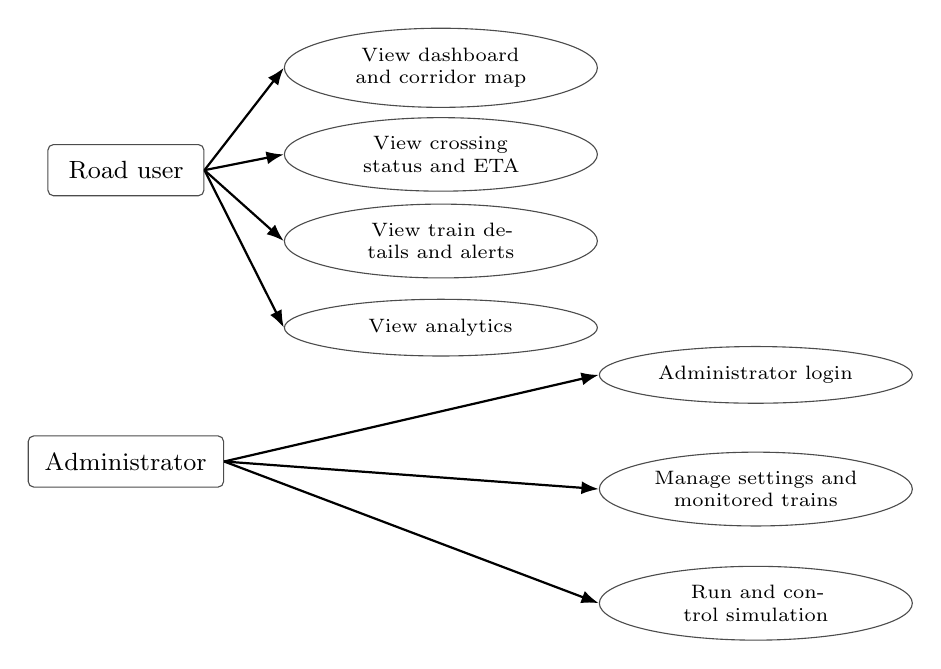
\begin{tikzpicture}
\node[actorbox] (viewer) at (0,0.7) {Road user};
\node[actorbox,minimum width=2.2cm,text width=2.2cm] (admin) at (0,-3.0) {Administrator};
\node[usecase] (dashboard) at (4,2.0) {View dashboard and corridor map};
\node[usecase] (crossing) at (4,0.9) {View crossing status and ETA};
\node[usecase] (trains) at (4,-0.2) {View train details and alerts};
\node[usecase] (analytics) at (4,-1.3) {View analytics};
\node[usecase] (login) at (8,-1.9) {Administrator login};
\node[usecase] (settings) at (8,-3.35) {Manage settings and monitored trains};
\node[usecase] (simulation) at (8,-4.8) {Run and control simulation};
\draw[arr] (viewer.east)--(dashboard.west);
\draw[arr] (viewer.east)--(crossing.west);
\draw[arr] (viewer.east)--(trains.west);
\draw[arr] (viewer.east)--(analytics.west);
\draw[arr] (admin.east)--(login.west);
\draw[arr] (admin.east)--(settings.west);
\draw[arr] (admin.east)--(simulation.west);
\end{tikzpicture}}
\caption{SmartCross use case diagram}
\label{fig:usecase}
\end{figure}

\section{Activity Diagram}
The activity diagram shows the live data processing path, including the fallback path when a usable live position is unavailable.

\begin{figure}[H]\centering
\resizebox{0.74\textwidth}{!}{%
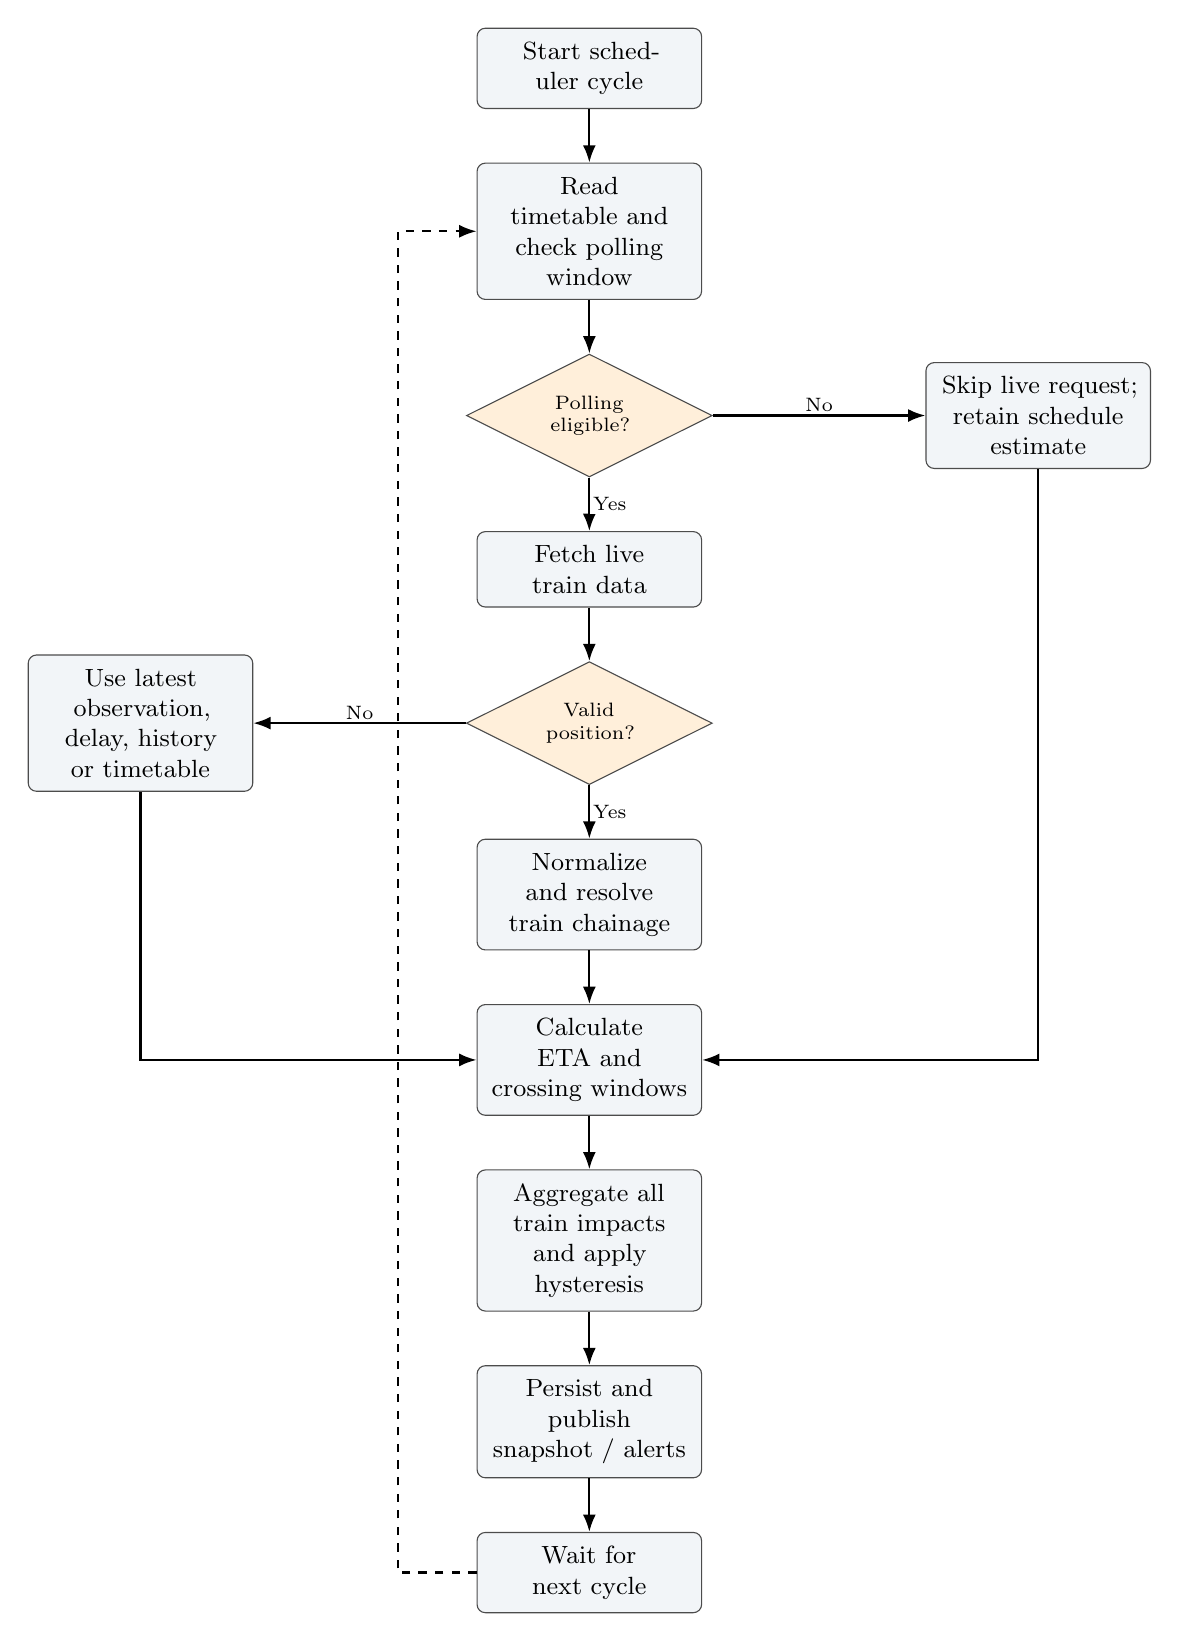
\begin{tikzpicture}[node distance=0.68cm]
\node[nodebox] (start) {Start scheduler cycle};
\node[nodebox,below=of start] (schedule) {Read timetable and\\check polling window};
\node[decision,below=of schedule] (eligible) {Polling eligible?};
\node[nodebox,below=of eligible] (fetch) {Fetch live train data};
\node[decision,below=of fetch] (valid) {Valid position?};
\node[nodebox,left=2.7cm of valid] (fallback) {Use latest observation,\\delay, history or timetable};
\node[nodebox,below=of valid] (resolve) {Normalize and resolve\\train chainage};
\node[nodebox,below=of resolve] (predict) {Calculate ETA and\\crossing windows};
\node[nodebox,below=of predict] (aggregate) {Aggregate all train impacts\\and apply hysteresis};
\node[nodebox,below=of aggregate] (publish) {Persist and publish\\snapshot / alerts};
\node[nodebox,below=of publish] (end) {Wait for next cycle};
\node[nodebox,right=2.7cm of eligible] (skip) {Skip live request;\\retain schedule estimate};
\draw[arr] (start)--(schedule);
\draw[arr] (schedule)--(eligible);
\draw[arr] (eligible)--node[labeltxt,right]{Yes}(fetch);
\draw[arr] (eligible)--node[labeltxt,above]{No}(skip);
\draw[arr] (skip) |- (predict);
\draw[arr] (fetch)--(valid);
\draw[arr] (valid)--node[labeltxt,right]{Yes}(resolve);
\draw[arr] (valid)--node[labeltxt,above]{No}(fallback);
\draw[arr] (fallback) |- (predict);
\draw[arr] (resolve)--(predict);
\draw[arr] (predict)--(aggregate);
\draw[arr] (aggregate)--(publish);
\draw[arr] (publish)--(end);
\draw[darr] (end.west) -- ++(-1.0,0) |- (schedule.west);
\end{tikzpicture}}
\caption{SmartCross live processing activity diagram}
\label{fig:activity}
\end{figure}

\section{Domain Class Diagram}
The diagram presents the principal domain objects and their logical relationships. It is a conceptual view of the implemented Mongoose models and services, not a literal class listing of every source file.

\begin{figure}[H]\centering
\resizebox{\textwidth}{!}{%
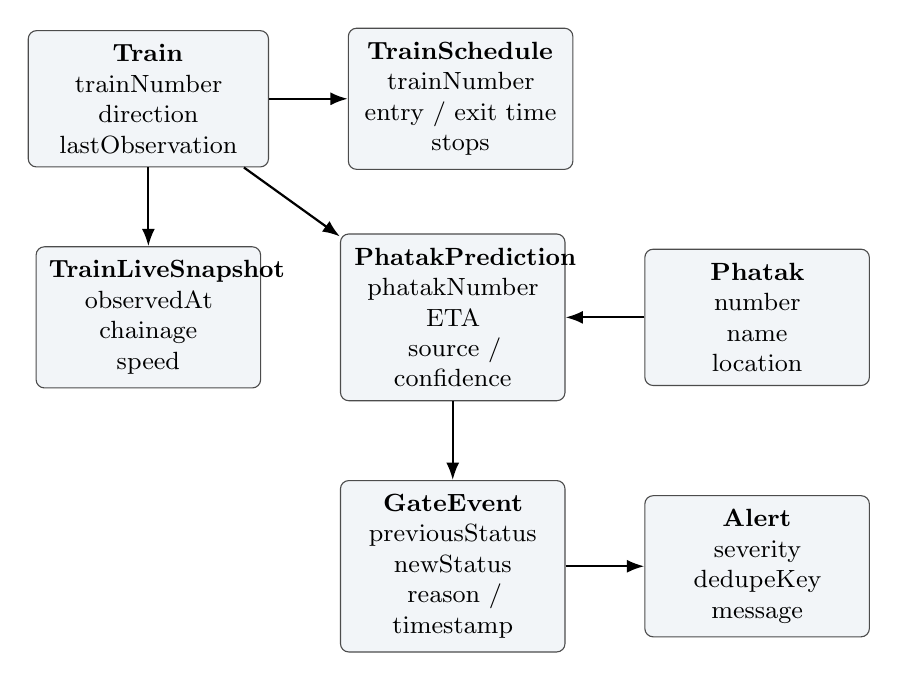
\begin{tikzpicture}[node distance=1.0cm and 1.0cm]
\node[nodebox,minimum width=2.6cm,text width=2.7cm] (train) {\textbf{Train}\\trainNumber\\direction\\lastObservation};
\node[nodebox,right=of train] (schedule) {\textbf{TrainSchedule}\\trainNumber\\entry / exit time\\stops};
\node[nodebox,below=of train] (snapshot) {\textbf{TrainLiveSnapshot}\\observedAt\\chainage\\speed};
\node[nodebox,right=of snapshot] (prediction) {\textbf{PhatakPrediction}\\phatakNumber\\ETA\\source / confidence};
\node[nodebox,right=of prediction] (phatak) {\textbf{Phatak}\\number\\name\\location};
\node[nodebox,below=of prediction] (event) {\textbf{GateEvent}\\previousStatus\\newStatus\\reason / timestamp};
\node[nodebox,right=of event] (alert) {\textbf{Alert}\\severity\\dedupeKey\\message};
\draw[arr] (train)--(schedule);
\draw[arr] (train)--(snapshot);
\draw[arr] (train)--(prediction);
\draw[arr] (phatak)--(prediction);
\draw[arr] (prediction)--(event);
\draw[arr] (event)--(alert);
\end{tikzpicture}}
\caption{Conceptual SmartCross domain class diagram}
\label{fig:class}
\end{figure}

\section{Software Development Life Cycle}
SmartCross follows an iterative development approach. Feedback from testing and simulation can lead to changes in requirements, design, implementation and test cases.

\begin{figure}[H]\centering
\resizebox{0.96\textwidth}{!}{%
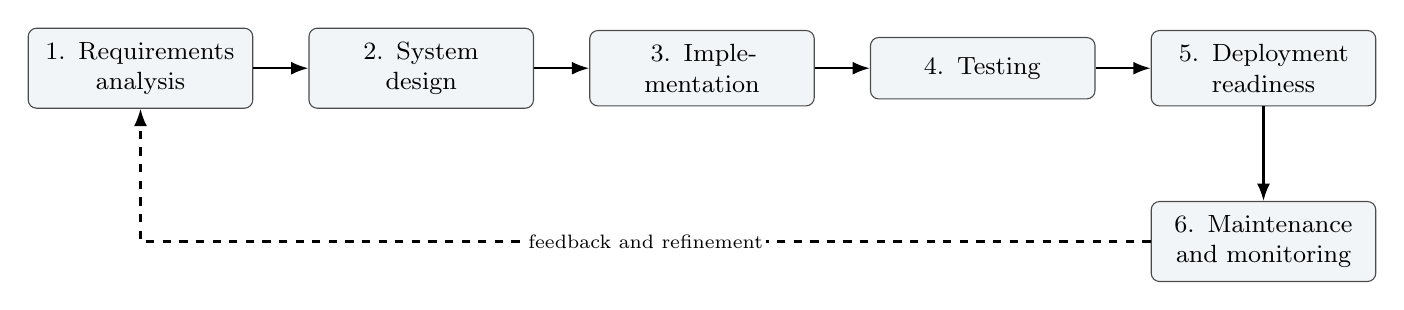
\begin{tikzpicture}[node distance=0.8cm and 0.7cm]
\node[nodebox] (req) {1. Requirements\\analysis};
\node[nodebox,right=of req] (design) {2. System\\design};
\node[nodebox,right=of design] (impl) {3. Implementation};
\node[nodebox,right=of impl] (test) {4. Testing};
\node[nodebox,right=of test] (deploy) {5. Deployment\\readiness};
\node[nodebox,below=1.2cm of deploy] (maint) {6. Maintenance\\and monitoring};
\draw[arr] (req)--(design);
\draw[arr] (design)--(impl);
\draw[arr] (impl)--(test);
\draw[arr] (test)--(deploy);
\draw[arr] (deploy)--(maint);
\draw[darr] (maint.west) -| node[labeltxt,pos=0.25]{feedback and refinement} (req.south);
\end{tikzpicture}}
\caption{Iterative SDLC followed for SmartCross}
\label{fig:sdlc}
\end{figure}

% CHAPTER 4
\chapter{Prediction and Crossing-State Methodology}
\section{Position Resolution and Chainage}
The project uses along-track distance rather than straight-line distance between a train and a crossing. A train position is resolved against the configured corridor geometry. RailRadar's documented live response provides route-distance information such as distance from the origin and station kilometre posts; the position resolver maps these values to the corridor chainage. An undocumented latitude/longitude value is not assumed to be available. If a coordinate is supplied, the resolver checks whether it is plausibly close to the track before using it.

For a crossing at chainage $s_c$ and a train at chainage $s_t$, the signed distance is determined using the train direction:
\[
D = (s_c-s_t)\times d
\]
where $d$ is the direction sign for the corridor. For a train moving towards the crossing, the resulting distance is positive.

\section{ETA Calculation}
A basic ETA estimate is:
\[
ETA_{\text{seconds}} = \frac{D_{\text{metres}}}{V_{\text{effective, m/s}}}
\]
The implementation uses an effective speed derived from measured and recent observed speeds, with historical or configured fallback speed where required. Speed is bounded to avoid division by zero and unrealistic estimates. The prediction also considers station dwell and a restart allowance for a train stopped between stations. Predictions beyond the configured maximum horizon are treated as unknown.

\section{Five-Level Prediction Fallback}
The prediction engine uses a hierarchy so that a missing live position does not automatically remove all useful information.

\begin{table}[H]\centering
\caption{Prediction source hierarchy}
\label{tab:fallback}
\begin{tabularx}{\textwidth}{c p{3.1cm} X c}
\toprule
\textbf{Level} & \textbf{Source} & \textbf{When it is used} & \textbf{Typical confidence}\\
\midrule
1 & LIVE\_POSITION & Fresh live position within the configured staleness threshold. & High / Medium\\
2 & LATEST\_OBSERVATION & Recent position retained for bounded dead reckoning. & Medium / Low\\
3 & TIMETABLE\_WITH\_DELAY & Timetable adjusted using a sufficiently recent observed delay. & Medium / Low\\
4 & HISTORICAL\_AVERAGE & Historical mean offset derived from sufficient observed live passages. & Medium / Low\\
5 & TIMETABLE\_ESTIMATE & Timetable-only interpolation when stronger sources are unavailable. & Low\\
-- & UNKNOWN & No acceptable source is available. & None\\
\bottomrule
\end{tabularx}
\end{table}

Confidence is reduced for stale observations and long prediction horizons. Each prediction carries its source, confidence, train number, calculation time, arrival estimate, ETA and predicted closure/reopening window.

\section{Adaptive Train Polling}
The timetable decides when live polling may start; live position determines the train's current movement and crossing ETA. The scheduler tracks trains from a configurable prediction look-ahead window. Live polling starts approximately 20 minutes before expected corridor entry and stops approximately 10 minutes after expected exit, subject to earlier completion when live data shows that the train has left.

The polling interval adapts to the next crossing ETA:
\begin{itemize}
  \item up to 5 minutes: approximately 45 seconds;
  \item up to 15 minutes: approximately 90 seconds;
  \item farther away or when a useful ETA is unavailable: approximately 180 seconds.
\end{itemize}
When the daily API budget becomes tight, intervals are stretched. When the budget is exhausted, polling is restricted to trains expected to reach a crossing within the priority window. The API client also applies caching, in-flight request de-duplication, request limits and handling for quota/authentication failures. These values are configuration-dependent and should be reviewed against the active RailRadar plan.

\section{Closure Window Estimation}
The system estimates a closure window from the train's predicted arrival, speed, configured closure distance/ETA thresholds, train length and clearance settings. The predicted reopening time is an estimate of when the train tail and clearance interval have passed the crossing. It is not a measurement of the actual barrier opening time.

\section{Gate State Machine}
The state machine translates train-level predictions into one predicted state for each crossing. The supported states are:
\begin{itemize}
  \item \textbf{OPEN:} no train is currently predicted to affect the crossing within the configured warning window.
  \item \textbf{CLOSING\_SOON:} a train is expected to reach the crossing soon.
  \item \textbf{CLOSED:} positional evidence indicates that a train is at/very near the crossing or the configured positional/ETA threshold is met.
  \item \textbf{OPENING\_SOON:} the train head has passed, but tail clearance is still pending.
  \item \textbf{UNKNOWN:} available information is insufficient for a reliable state.
\end{itemize}

A key safety rule in the implementation is that timetable-only and historical-only estimates may warn that a train is expected, but they cannot independently assert the CLOSED state. A CLOSED prediction requires positional evidence. This prevents a timetable estimate from being presented as confirmation of a physical closure.

\begin{figure}[H]\centering
\resizebox{0.92\textwidth}{!}{%
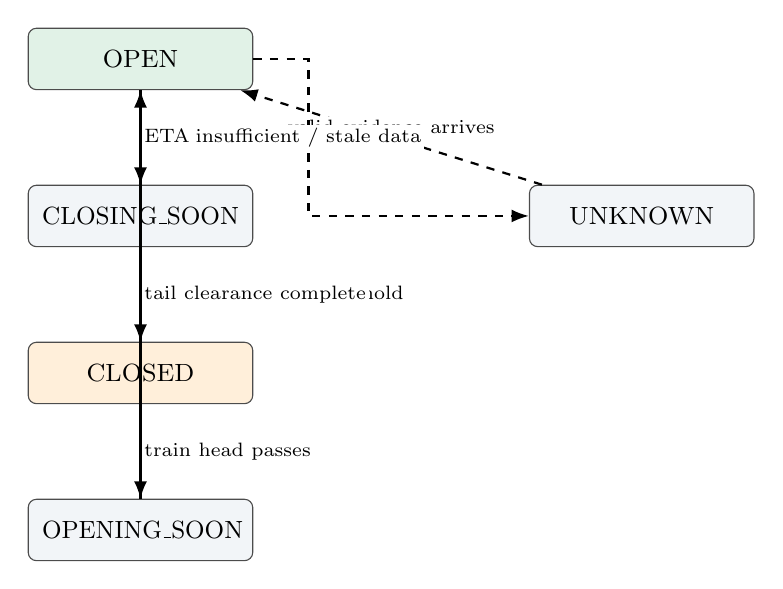
\begin{tikzpicture}[node distance=1.2cm and 1.4cm]
\node[nodebox,fill=scgreen] (open) {OPEN};
\node[nodebox,below=of open] (closing) {CLOSING\_SOON};
\node[nodebox,below=of closing,fill=scorange] (closed) {CLOSED};
\node[nodebox,below=of closed] (opening) {OPENING\_SOON};
\draw[arr] (open)--node[labeltxt,right]{ETA enters warning window}(closing);
\draw[arr] (closing)--node[labeltxt,right]{positional / near threshold}(closed);
\draw[arr] (closed)--node[labeltxt,right]{train head passes}(opening);
\draw[arr] (opening)--node[labeltxt,right]{tail clearance complete}(open);
\node[nodebox,right=3.5cm of closing] (unknown) {UNKNOWN};
\draw[darr] (unknown)--node[labeltxt,above]{valid evidence arrives}(open);
\draw[darr] (open.east) -- ++(0.7,0) |- node[labeltxt,pos=0.25]{insufficient / stale data}(unknown);
\end{tikzpicture}}
\caption{Predicted crossing-state lifecycle}
\label{fig:state}
\end{figure}

\section{Multiple Trains, Grouped Closures and Hysteresis}
The engine evaluates every relevant train for each crossing. It applies a state priority so that one train passing cannot cause a crossing to be shown OPEN while another train is still approaching. Opposite-direction and back-to-back trains are handled by aggregating their predicted impacts. If the next positional train's predicted closure begins within the configured gap from the preceding reopening, the crossing may remain predicted CLOSED.

Group A (19 and 20) and Group B (23 and 24) are analysed for sequential effects. Each crossing retains its own arrival and closure window; the grouped advisory reports whether the predicted windows overlap. Hysteresis prevents rapid state changes: escalations and passage-driven transitions are applied immediately, while selected downgrades must persist for the configured confirmation duration before they are accepted.

% CHAPTER 5
\chapter{Database and Application Design}
\section{Database Design}
MongoDB is used for persistence. The project defines Mongoose models for crossing reference data, trains, schedules, routes, live snapshots, predictions, historical observations, alerts, state-transition events, settings and audit information.

\begin{longtable}{p{4.0cm}p{9.5cm}}
\toprule
\textbf{Model / Collection} & \textbf{Purpose}\\
\midrule
Phatak & Crossing reference information and latest predicted state.\\
Train & Monitored train metadata and latest live observation.\\
TrainSchedule & Timetable information for monitored trains.\\
TrainRoute & Route stops, kilometre posts and route geometry.\\
TrainLiveSnapshot & Time-stamped live observations, with deduplication and retention.\\
TrainPhatakMapping & Mapping of a train to its relevant crossings and direction.\\
PhatakPrediction & Current per-mode, per-train, per-crossing prediction.\\
Prediction & Prediction samples at configured time horizons.\\
PredictionEvaluation & Comparison of predicted and observed arrival information.\\
HistoricalTrainObservation & Historical positional observations used for learning and evaluation.\\
GateEvent & Predicted crossing-state transitions with source, confidence and reason.\\
Alert & Gate-state, grouped-closure and system-warning alerts.\\
NotificationSubscription & Browser notification preferences.\\
SystemSetting & Runtime thresholds and monitored train configuration.\\
AuditLog & API usage and administrator/system audit records.\\
\bottomrule
\end{longtable}

\section{Entity Relationship Overview}
Figure~\ref{fig:erd} shows the logical relationships. It is an overview of the principal data entities; MongoDB stores documents and references rather than enforcing relational foreign keys.

\begin{figure}[H]\centering
\resizebox{\textwidth}{!}{%
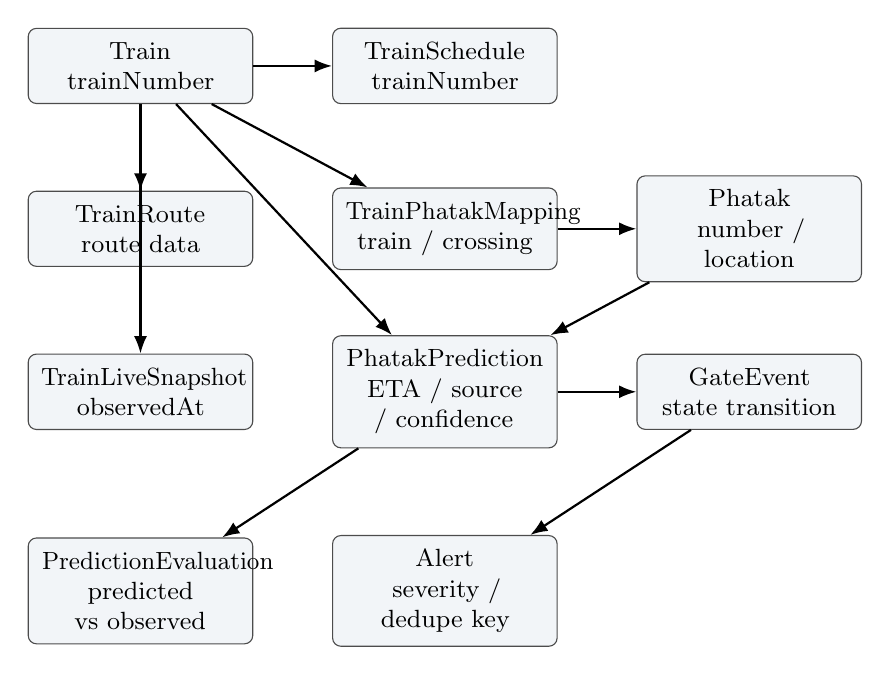
\begin{tikzpicture}[node distance=1.1cm and 1.0cm]
\node[nodebox] (train) {Train\\trainNumber};
\node[nodebox,right=of train] (sched) {TrainSchedule\\trainNumber};
\node[nodebox,below=of train] (route) {TrainRoute\\route data};
\node[nodebox,right=of route] (mapping) {TrainPhatakMapping\\train / crossing};
\node[nodebox,right=of mapping] (phatak) {Phatak\\number / location};
\node[nodebox,below=of route] (snap) {TrainLiveSnapshot\\observedAt};
\node[nodebox,right=of snap] (pred) {PhatakPrediction\\ETA / source / confidence};
\node[nodebox,right=of pred] (event) {GateEvent\\state transition};
\node[nodebox,below=of pred] (alert) {Alert\\severity / dedupe key};
\node[nodebox,left=of alert] (eval) {PredictionEvaluation\\predicted vs observed};
\draw[arr] (train)--(sched);
\draw[arr] (train)--(route);
\draw[arr] (train)--(snap);
\draw[arr] (train)--(mapping);
\draw[arr] (mapping)--(phatak);
\draw[arr] (train)--(pred);
\draw[arr] (phatak)--(pred);
\draw[arr] (pred)--(event);
\draw[arr] (event)--(alert);
\draw[arr] (pred)--(eval);
\end{tikzpicture}}
\caption{Logical data relationship diagram}
\label{fig:erd}
\end{figure}

\section{Frontend Modules}
The React application contains the following pages and shared components:
\begin{itemize}
  \item \textbf{Dashboard:} corridor overview, crossing cards and current system snapshot.
  \item \textbf{Map:} map-based view of the monitored corridor, trains and crossings.
  \item \textbf{Trains and Train Detail:} monitored train list, train status, direction and predictions.
  \item \textbf{Crossing Detail:} crossing-specific state, contributing trains, ETA and history.
  \item \textbf{Alerts:} alert history and notification preferences.
  \item \textbf{Analytics:} frequency, speed, waiting estimates, prediction evaluation and API usage.
  \item \textbf{Admin and Settings:} protected configuration, monitoring and operational controls.
  \item \textbf{Simulation:} predefined and custom multi-train scenarios.
\end{itemize}

\section{REST API and Real-Time Communication}
The backend exposes REST endpoints under \texttt{/api}. Public read endpoints provide health, state, corridor, phatak, train, prediction, alert and analytics information. Protected administrator endpoints support login, settings changes, mode control, API logs, scheduler status, manual refresh and simulation control.

Socket.IO is used for real-time communication. Important events include:
\begin{itemize}
  \item \texttt{corridor:snapshot}: complete state snapshot with sequence number;
  \item \texttt{train:update} and \texttt{phatak:update}: entity-specific updates;
  \item \texttt{gate:status-change}: predicted crossing-state transition;
  \item \texttt{alert:new}: newly created alert;
  \item \texttt{system:status}: operating-mode or system-status update.
\end{itemize}
The frontend can request a fresh snapshot after reconnecting. Sequence numbers help the client discard duplicate or out-of-order updates.

% CHAPTER 6
\chapter{Implementation}
\section{Backend Implementation}
The backend is implemented with Node.js and Express. The entry point connects to MongoDB, seeds reference data, loads settings, initializes Socket.IO, selects the operating mode, starts the corridor engine and scheduler, and supports graceful shutdown.

The implementation separates controllers and routes from domain services. The runtime module wires the engine, scheduler, simulation, Socket.IO manager and RailRadar client. This separation allows prediction and state-machine logic to be tested independently of HTTP transport.

\section{RailRadar Integration}
The RailRadar client is responsible for authenticated requests, timeouts, bounded retries, caching, in-flight request de-duplication and quota/rate-limit handling. Live responses are normalized before being ingested by the engine. If the API key is not configured, the application can start in simulation mode rather than presenting simulated data as live data.

\section{Simulation Implementation}
The simulation engine supports predefined scenarios including:
\begin{enumerate}
  \item single train from Patiala towards Dhablan;
  \item single train from Dhablan towards Patiala;
  \item grouped closure affecting Group B and then Group A;
  \item opposing trains;
  \item back-to-back trains in the same direction;
  \item delayed departure / station hold; and
  \item live-position loss followed by dead reckoning.
\end{enumerate}
Custom simulated trains can be configured with direction, speed, starting position, delay, hold and optional signal loss. The simulation provider produces RailRadar-format mock payloads and feeds them through the same normalizer and prediction engine. Simulation data is labelled separately throughout the application.

\section{Alert Generation}
Alerts are generated from actual predicted state transitions, grouped-closure advisories and system warnings. A deduplication key and cooldown suppress repeated identical alerts. Alerts are persisted where possible and emitted to connected clients. Alert wording identifies the status as predicted and may include the data source and confidence.

\section{Security and Operational Controls}
The project includes administrator authentication using a password-based login flow and JWT-protected operations, request validation, rate limiting, CORS configuration, security headers, centralized error handling and environment-based configuration. API keys and secrets are intended to remain in backend environment variables and are not sent to the frontend. Production use requires strong administrator credentials, a strong JWT secret, a production MongoDB URI and a restricted client-origin configuration.

% CHAPTER 7
\chapter{Testing and Evaluation}
\section{Testing Strategy}
The project includes automated backend tests using Jest and integration tests using Supertest and Socket.IO clients. The repository documentation describes a suite of 132 backend tests across 13 test suites. The source archive contains tests for the following areas:
\begin{itemize}
  \item GIS coordinate conversion, corridor ordering, chainage and position resolution;
  \item RailRadar response normalization and API-client behaviour;
  \item ETA calculation, fallback prediction and ETA smoothing;
  \item gate-state transitions, hysteresis, multiple trains and grouped closures;
  \item corridor-engine behaviour, stale data and mode separation;
  \item simulation scenarios and validation;
  \item adaptive scheduler timing, polling intervals and quota handling;
  \item REST API and Socket.IO integration.
\end{itemize}

The count above is the test-suite count documented in the supplied project README. It should not be interpreted as a claim that tests were executed successfully during preparation of this report. The final submission team should run the test command and record the actual pass/fail output on the submission machine.

\section{Representative Test Cases}
\begin{longtable}{p{1.2cm}p{4.1cm}p{6.8cm}p{1.5cm}}
\toprule
\textbf{ID} & \textbf{Test area} & \textbf{Expected behaviour} & \textbf{Evidence}\\
\midrule
TC-01 & Corridor geometry & Crossing order and chainage resolve consistently along the track. & Automated test\\
TC-02 & Live response normalization & Valid response is normalized; invalid or mismatched payload is rejected safely. & Automated test\\
TC-03 & ETA calculation & ETA uses distance and bounded effective speed; zero speed does not cause division by zero. & Automated test\\
TC-04 & Fallback prediction & Each supported source level is selected under its documented conditions. & Automated test\\
TC-05 & Stale position & Prediction degrades to a lower-confidence source when observation becomes stale. & Automated test\\
TC-06 & State progression & A simulated train produces OPEN, CLOSING\_SOON, CLOSED, OPENING\_SOON and OPEN transitions. & Automated test\\
TC-07 & Timetable-only rule & Timetable-only prediction does not assert CLOSED. & Automated test\\
TC-08 & Opposing trains & A crossing is not shown OPEN while another train still affects it. & Automated test\\
TC-09 & Back-to-back trains & Overlapping predicted closure windows are aggregated without a false opening. & Automated test\\
TC-10 & Polling schedule & Live polling begins and ends within the configured timetable window. & Automated test\\
TC-11 & Quota handling & Polling respects daily budget and API rate-limit responses. & Automated test\\
TC-12 & Simulation mode & Simulation data is kept separate from live data and does not trigger live polling. & Automated test\\
TC-13 & Socket.IO & Connected clients receive snapshots and relevant state/alert events. & Integration test\\
TC-14 & API validation & Invalid requests return controlled error responses. & Integration test\\
\bottomrule
\end{longtable}

\section{Evaluation Metrics}
The implementation exposes or records data that can support the following evaluation metrics. Actual numerical performance results must be taken from a real test run or recorded analytics; they are not fabricated in this report.

\begin{table}[H]\centering
\caption{Evaluation metrics and measurement method}
\label{tab:metrics}
\begin{tabularx}{\textwidth}{p{3.0cm}X p{3.5cm}}
\toprule
\textbf{Metric} & \textbf{Measurement method} & \textbf{Current report value}\\
\midrule
API response latency & Measure request start-to-response time for representative endpoints. & To be measured\\
Prediction processing time & Measure time taken by corridor evaluation for a snapshot. & To be measured\\
ETA error & Compare predicted arrival with observed passage at the same crossing. & To be measured from recorded observations\\
State transition correctness & Compare simulated/observed event sequence with expected state progression. & Covered by automated test cases; execution result to be recorded\\
Polling efficiency & Compare API calls with the configured schedule and quota budget. & To be measured from API logs\\
Real-time delivery delay & Measure event creation time to client receipt time. & To be measured\\
System availability & Monitor successful health checks over a defined period. & To be measured\\
\bottomrule
\end{tabularx}
\end{table}

\section{Known Limitations}
\begin{enumerate}
  \item The system has no physical gate sensors; displayed crossing states are predictions.
  \item Coverage is limited to configured monitored passenger trains; freight and unscheduled trains are outside the current prediction scope.
  \item Prediction quality depends on the availability, freshness and correctness of RailRadar and timetable data.
  \item Historical prediction quality improves only as sufficient real positional observations are collected.
  \item Closure and reopening thresholds are configurable software assumptions, not verified railway operating timings.
  \item Real-world ETA accuracy, latency and availability must be established through field data and measured evaluation.
\end{enumerate}

% CHAPTER 8
\chapter{Results, Discussion and Future Work}
\section{Implemented Outcomes}
The supplied source code and project documentation show that SmartCross has progressed beyond a basic train-location display. The implementation contains:
\begin{itemize}
  \item a four-crossing corridor configuration with track-relative chainage;
  \item timetable-aware adaptive polling and RailRadar API quota controls;
  \item a normalizer and position resolver for external train observations;
  \item a five-level fallback prediction hierarchy and ETA smoothing;
  \item a multi-train crossing aggregation engine with hysteresis;
  \item grouped-closure advisories for the two crossing groups;
  \item LIVE and SIMULATION modes using a common processing pipeline;
  \item REST APIs, Socket.IO updates, alerts, analytics and administration pages; and
  \item automated unit and integration test coverage for core backend behaviour.
\end{itemize}

These outcomes demonstrate the integration of external data, geospatial processing, prediction logic, persistence and real-time user-interface updates. They do not, by themselves, establish field-level accuracy or operational safety certification.

\section{Discussion}
The most important design decision is to distinguish a predicted state from a physically confirmed gate state. The fallback hierarchy also makes the system more resilient: it can continue to provide lower-confidence timetable-based warnings when live positions are unavailable, while preventing timetable-only information from asserting CLOSED. Multi-train aggregation and hysteresis reduce misleading state changes when trains approach from different directions or follow one another closely.

The simulation engine is useful because it exercises the same processing pipeline with controlled conditions. However, simulated results validate software behaviour under the chosen scenarios; they do not replace validation against real train and crossing observations.

\section{Future Work}
\begin{enumerate}
  \item Collect a larger, verified dataset of real train passages and actual crossing closure/opening observations.
  \item Calibrate closure distance, clearance and reopening assumptions using railway-authority data where available.
  \item Evaluate ETA error by crossing, train, direction, prediction horizon and data source.
  \item Extend monitored corridor coverage only after verifying track geometry, train schedules and crossing references.
  \item Improve resilience through additional trusted train-data providers, where permitted.
  \item Conduct controlled user testing for alert clarity, accessibility and the interpretation of prediction confidence.
  \item Perform security, load and deployment testing in a production-like environment.
\end{enumerate}

% CHAPTER 9
\chapter{Conclusion}
SmartCross is a real-time railway-crossing information and prediction application for the Patiala--Dhablan corridor. It combines timetable-aware train tracking, RailRadar live observations, track-relative position resolution, ETA estimation, fallback prediction sources, multi-train state aggregation and real-time communication through a web application.

The implementation includes four configured crossings, two grouped-closure areas, a MongoDB persistence layer, administrative controls, analytics, alert generation and a simulation environment. Its modular design supports testing and future extension.

The system must be understood as a decision-support and information tool. Since it does not receive physical gate-sensor readings or control railway infrastructure, all displayed crossing states and waiting times remain estimates. Further real-world data collection, accuracy evaluation and operational validation are necessary before any safety-critical deployment.

\chapter*{References}
\addcontentsline{toc}{chapter}{References}
\begin{enumerate}
  \item SmartCross project source code and README documentation supplied with this evaluation.
  \item RailRadar API endpoints and response fields referenced by the SmartCross integration.
  \item OpenStreetMap railway geometry used to construct the corridor track reference.
  \item Node.js and Express.js documentation: \url{https://nodejs.org/} and \url{https://expressjs.com/}.
  \item React documentation: \url{https://react.dev/}.
  \item MongoDB documentation: \url{https://www.mongodb.com/docs/}.
  \item Socket.IO documentation: \url{https://socket.io/docs/v4/}.
\end{enumerate}

\appendix
\chapter{Suggested Commands for Reproducible Verification}
The repository README documents the following commands. Run them from the project directory in the appropriate environment and retain the terminal output as evaluation evidence.

\begin{verbatim}
# Install dependencies
npm run install:all

# Start backend and frontend in separate terminals
npm run dev:backend
npm run dev:frontend

# Run backend automated tests
cd backend
npm test

# Verify configured crossing coordinates
npm run verify-coords
\end{verbatim}

\chapter{Submission Verification Checklist}
Before final submission, the project team should:
\begin{enumerate}
  \item Run the backend test suite and record the actual passed, failed and skipped counts.
  \item Capture screenshots of the dashboard, corridor map, crossing details, alerts, analytics, admin and simulation pages.
  \item Record measured API latency and prediction-processing time rather than entering estimated values.
  \item Clearly label screenshots and test data as LIVE or SIMULATION.
  \item Ensure no API keys, passwords, JWT secrets or private environment files are included in the submission archive.
  \item Verify that the final PDF compiles from this exact LaTeX source.
\end{enumerate}
\end{document}
